\documentclass[11pt]{article}

\usepackage{graphicx,natbib,setspace,lineno}
\usepackage{amsmath,wasysym,fullpage}

\renewcommand{\thefootnote}{$\star$}

\title{Geochronology of Taung and other southern African australopiths}

\author{Pieter Vermeesch\\
  University College London, Gower Street\\
  London WC1E 6BT\\
  \texttt{p.vermeesch [at] ucl.ac.uk}\\~\\
  Philip Hopley \\
  Birkbeck, University of London, Malet Street\\
  London WC1E 7HX\\
  \texttt{p.hopley [at] ucl.ac.uk}\\~\\
  Nick Roberts \\
  British Geological Survey, Keyworth\\
  Nottingham NG12 5GG \\
  \texttt{nirob [at] bgs.ac.uk}\\~\\
  Randall Parrish \\
  University of Portsmouth\\
  Portsmouth PO1 3QL\\
  \texttt{randall.parrish [at] port.ac.uk}
  }

%\onehalfspacing

%\linenumbers

\begin{document}


\maketitle

\begin{abstract}
  One century after the Taung juvenile's discovery, its age and that
  of many other southern African australopiths remains unknown.  This
  lack of accurate geochronological constraints leaves important
  questions unanswered, including the temporal relationship between
  the South African fossil sites and their well dated eastern African
  counterparts.  Previous age estimates for the Taung fossil range
  from 942\,ka to 3.03\,Ma. Radiometric age estimation is difficult in
  the absence of the volcanic marker beds that are so useful in
  eastern Africa. The advent of carbonate U--Pb geochronology has been
  heralded as the long-awaited solution to this conundrum. However,
  some notes of caution are necessary, because the
  \textsuperscript{206}Pb/\textsuperscript{238}U isochron method
  requires correction for any initial
  \textsuperscript{234}U/\textsuperscript{238}U disequilibrium. In the
  case of southern African carbonates, this correction sometimes
  exceeds 50\%. We show that, beyond $\sim{1.5}$\,Ma, the uncertainty
  of the disequilibrium correction may exceed the correction itself,
  degrading the value of the
  \textsuperscript{206}Pb/\textsuperscript{238}U method.  We propose
  the \textsuperscript{207}Pb/\textsuperscript{235}U method as an
  alternative to the \textsuperscript{206}Pb/\textsuperscript{238}U
  method, because it is largely unaffected by initial disequilibrium.
  We use this alternative U--Pb dating approach to obtain a new
  minimum age estimate for the Taung juvenile, by analysing a
  flowstone situated above, and in stratigraphic succession with, the
  fossil-bearing deposit.  The uncorrected
  \textsuperscript{206}Pb/\textsuperscript{238}U isochron age for the
  sample is $3.30\pm{0.12}$\,Ma. Disequilibrium correction lowers this
  value to $2.05+0.11/-0.08$\,Ma, a correction of 40\%. The
  \textsuperscript{207}Pb/\textsuperscript{235}U isochron age of
  $2.982\pm{0.057}$\,Ma is close to the uncorrected
  \textsuperscript{206}Pb/\textsuperscript{238}U age. Unfortunately,
  the two age estimates do not overlap within uncertainty. We
  attribute this disagreement to open system behaviour of the uranium
  in the sample, which leads to an overestimation of the
  \textsuperscript{234}U/\textsuperscript{238}U disequilibrium
  correction and an underestimation of the
  \textsuperscript{207}Pb/\textsuperscript{235}U isochron age.
  Consequently, the \textsuperscript{207}Pb/\textsuperscript{235}U
  isochron age of $\sim{3}$\,Ma is a minimum age estimate for the
  flowstone and for the Taung juvenile, placing both firmly in the
  Pliocene epoch. Disappointingly, LA-ICP-MS screening of borehole
  samples below the Taung discovery site have not yielded any further
  datable carbonates. Therefore, we have not been able to pair our
  minimum age estimate with an equally robust upper age bracket. The
  search for this additional age constraint continues.
\end{abstract}

\section{Introduction}\label{sec:intro}

The scientific importance of the Taung juvenile (hereafter Taung) can
hardly be overstated. It is the holotype of \emph{Australopithecus
africanus} and provided the first evidence for Charles Darwin's
assertion that humans evolved in Africa \citep{dart1925}. But despite
its importance and 100~years of research, the age of the fossil is
frustratingly poorly constrained. This is due to a combination of at
least five reasons:

\textbf{The Plio-Pleistocene geochronology conundrum.} The
Plio-Pleistocene falls in an awkward `dating gap' between young events
($<50\,$ka) that can be dated with radiocarbon, and older parts of the
geologic timescale ($>5\,$Ma), where long-lived radionuclides such as
\textsuperscript{238}U and \textsuperscript{40}K can be routinely
used  \citep{isaac1975}.

Nevertheless, the burgeoning field of Quaternary geochronology has
produced a number of breakthrough technologies that generate robust
Plio-Pleistocene age constraints. Arguably the most successful of
these techniques is ${}^{40}$Ar/${}^{39}$Ar-dating of volcanic
ash. This method has provided precise and accurate time constraints on
human evolution in eastern Africa \citep{deino2023}. Unfortunately, it
is not applicable to southern Africa, for reasons we discuss.

\textbf{Geological setting.} Famous eastern African hominin discovery
sites, such as the Omo-Turkana Basin and Olduvai (now Oldupai), are
situated in the eastern African rift system (EARS), an area of active
volcanism. This geological setting creates the ideal conditions for
accurate chronostratigraphy. Many eastern African hominin fossils are
found in fluviolacustrine deposits intercalated with volcanic ash
layers amenable to K--Ar and ${}^{40}$Ar/${}^{39}$Ar dating
\citep{leakey1961,deino2023}.

Unfortunately, the EARS terminates in Malawi and no recent volcanic
activity is found south of that. Therefore, the
${}^{40}$Ar/${}^{39}$Ar method is not applicable to southern African
hominins and other, less straightforward techniques must be used.

Whereas eastern African hominin fossils are generally found in
siliciclastic deposits, many southern African specimens were
discovered in carbonate lithologies (caves and tufa deposits).  Until
recently, the two dominant techniques to determine the age of these
rocks were terrestrial cosmogenic nuclide (TCN) geochronology of
siliciclastic cave fill \citep[e.g.,][]{partridge2003, granger2015,
  kramers2017, granger2022} and Th/U disequilibrium dating of
speleothems, or of the fossils themselves \citep[e.g.,][]{vogel1984,
  grun2023}. The Th/U disequilibrium dating method has an age limit of
$\sim{500}\,$ka and is sensitive to U-migration, which can be
triggered by changes in redox state \citep{tobias1993,ivanovich1994}.
In recent years, the carbonate U--Pb method has gained significant
popularity as a replacement for TCN and Th/U disequilibrium dating
\citep{walker2006,dirks2010,pickering2019}.

\textbf{Inconsistent results.} Unfortunately, the U--Pb results are
inconsistent with previously obtained TCN dates. Whereas the TCN dates
of southern African australopiths are similar to the ages of their
eastern African counterparts, their U--Pb dates are systematically
younger by $\sim$1\,Ma (Section~\ref{sec:EastVsSouth}). Complex
sedimentological arguments have been developed to reconcile these
differences, either by arguing that the cosmogenic nuclide dates are
too old \citep{kramers2017}, or that the U--Pb dates are too young
\citep{bruxelles2019,granger2022}.

\textbf{Unknown discovery location.} The previous three problems apply
to all southern African hominins. The situation is further complicated
for Taung because the exact location of its discovery is unknown.  The
skull was found by a quarry worker \citep[`Mr. de
  Bruyn';][]{tobias1984, tobias2000} in the Buxton-Norlim
limeworks. By the time its scientific value was recognised, the
quarrying had progressed beyond the discovery site. Quarrying
continued until until the 1970s, removing most geological evidence
except for two `pinnacles' that were left standing near the discovery
site thanks to the foresight of the quarry manager.

These pinnacles were named after Raymond Dart (the anatomist who
recognised that Taung was a hominin and not a baboon) and Ale\v{s}
Hrdli\v{c}ka (who carried out an early expedition to Taung in
1925). Our current understanding of the Taung stratigraphy is mostly
based on the Dart and Hrdli\v{c}ka pinnacles and the shallow
subsurface beneath them.

\textbf{Geographic isolation.} In the absence of reliable radiometric
age constraints, biostratigraphic correlations with other hominin
discovery sites offer an alternative approach to constraining geologic
time.  Unfortunately, such correlations are difficult for Taung, not
only because its stratigraphic context is poorly preserved (see the
previous point), but also because the site is geographically isolated
from other hominin discovery sites. Taung is located near the edge of
the Kalahari desert in the present day and it experiences more arid
conditions than the Cradle of Humankind. If similar climatic and
ecological gradients were present in the Plio-Pleistocene, they may
complicate biological correlations between these two regions
\citep{mckee1993}.

The coincidence of the above five problems explains why the age of
Taung is so poorly constrained, with estimates ranging from 1 to
3\,Ma. Section~\ref{sec:review} will review these existing estimates
and will explain in more detail why none of them are entirely
reliable. Section~\ref{sec:UPb-method} will review the carbonate U--Pb
dating method, which has been proposed as a potential solution to the
southern African hominin dating conundrum \citep{woodhead2012}. We
will show that this technique has issues of its own, which lead us to
conclude that the accuracy and precision of several published hominin
dates has been overestimated.

Fortunately, there is hope for a better solution.
Section~\ref{sec:UPb-results} will advocate the
${}^{207}$Pb/${}^{235}$U method as a more accurate approach to U--Pb
geochronology than the established ${}^{206}$Pb/${}^{238}$U method. We
will use this new flavour of U--Pb geochronology to obtain a robust
minimum age estimate for Taung of $\sim{3}\,$Ma.  The new estimate is
considerably older than the disequilibrium-corrected
${}^{206}$Pb/${}^{238}$U age, and closer to the ages of
broadly-equivalent eastern African australopiths than other southern
African hominin age estimates (Section~\ref{sec:EastVsSouth}).

\section{Wider context: conflicting chronologies for \emph{Australopithecus}}
\label{sec:EastVsSouth}

\emph{Australopithecus} in southern Africa is represented by at least
two endemic species, \emph{Australophithecus africanus} and
\emph{Australopithecus sediba}; the latter is known from palaeokarst
locality Malapa, dated by U--Pb methods and magnetostratigraphy to
2.0\,Ma \citep{pickering2011a}.  \emph{Australopithecus africanus} is
known from four localities: Sterkfontein, Gladysvale, Makapansgat, and
Taung.

\emph{Australopithecus africanus} material has been retrieved from
Sterkfontein Members~2 and 4; sediment from Member 2 has been dated to
$3.67 \pm 0.16$\,Ma \citep{granger2015} and from Member~4 to between
3.6 and 3.4\,Ma \citep{granger2022} using cosmogenic
\textsuperscript{10}Be/\textsuperscript{26}Al burial dating. These
dates conflict with flowstone U--Pb ages of $\sim$2.2\,Ma from
Member~2 \citep{walker2006,pickering2019} and 2.8--2.0\,Ma from
Member~4 \citep{pickering2010,pickering2019}; some explain this
discrepancy by arguing that two-stage burial processes have produced
excessively old cosmogenic ages \citep{kramers2017}; others have
argued that the flowstones are stratigraphically `intrusive', and
post-date the hominin fossils \citep{bruxelles2019}.

\emph{Australopithecus africanus} from Gladysvale \citep{berger1993a}
is represented by two isolated teeth collected from an ex-situ lime
dump and dated to approximately 2\,Ma on the basis of biostratigraphic
inference \citep{berger1993b}. Fossil hominins from Makapansgat,
assigned by some to \emph{Australopithecus africanus},
\citep{berger2019c} and others to \emph{Australopithecus prometheus}
\citep{clarke2019} are dated to between 2.5--2.0\,Ma using
palaeomagnetic and biostratigraphic inferences. A recent study uses
fossil cercopithecid biochronology \citep{frost2022} to suggest that
there are no hominin sites in southern Africa older than
$\sim$2.8\,Ma. This implies that the Sterkfontein Member~2 and 4
cosmogenic isotope ages are incorrect, but does not explain why this
might be. Unfortunately, all this means that presently no
\emph{Australopithecus africanus} fossils are associated with
well-accepted and fully quantitative radiometric ages.

Despite the many chronological uncertainties associated with
\emph{Australopithecus} in southern Africa, it is often considered
necessary to incorporate best-estimate chronological information
(first and last appearance date; FAD and LAD) for
\emph{Australopithecus africanus} and \emph{Australopithecus sediba}
into hominin evolutionary analyses.  Due to the above dating
controversies, \emph{Australopithecus africanus} is either given a
maximum stratigraphic range (e.g. from 3.8 to 2.0\,Ma) or a minimum
stratigraphic range (e.g. 3.0 to 2.4\,Ma); with many variations
existing in the literature
\citep[e.g.][]{wood2016,vanholstein2022,vanholstein2024,puschel2021,mongle2022}. For
\emph{Australopithecus sediba}, with just one geological horizon
available, the FAD and LAD are identical, and a number of statistical
approaches are available to take this stratigraphic and sampling
uncertainty into account \citep[e.g.][]{hopley2022b,vanholstein2024}.

When the full age uncertainty is considered (3.8 to 2.0\,Ma),
\emph{Australopithecus africanus} has the longest stratigraphic range
of all fossil hominins, with the possible exception of \emph{Homo
erectus} \citep[e.g.][]{wood2016}. This stratigraphic range exceeds
that of the combined \emph{Australopithecus anamensis} (4.2--3.9\,Ma)
and \emph{Australopithecus afarensis} (3.7--3.0\,Ma) anagenetic
pairing, a far more abundant and well-dated collection of
fossils. Either \emph{Australopithecus africanus} was an unusually
long-lived species, or poor dating accuracy and precision have
resulted in an artificially expanded stratigraphic range.

With the exception of the single occurrence of the enigmatic
\emph{Australopithecus garhi} at 2.5\,Ma \citep{asfaw1999} from the
Bouri Formation of Ethiopia, the youngest occurrence of
\emph{Australopithecus} outside of South Africa is
\emph{Australopithecus afarensis} at 3.0\,Ma from Hadar, Ethiopia
\citep{alemseged2005}. If the southern African australopiths are
indeed younger than 3.0\,Ma \citep[as suggested by the most recent
  biostratigraphic inferences of][]{frost2022}, then this represents a
relict population following eastern African extirpation. An equally
plausible scenario is that southern African and eastern African
\emph{Australopithecus} are broadly contemporaneous (from 4.0 to 3.0
Ma), as implied by the cosmogenic isotope ages of \citet{granger2022},
and that the current U--Pb and electron spin resonance (ESR) age
estimates from southern Africa are too young
(Figure~\ref{fig:EastVsSouth}a).

In a first attempt to reconcile the differences between the cosmogenic
burial dates and the carbonate U--Pb dates, we re-calculated the
latter from the raw isotopic ratio data reported in the literature
(see Section~\ref{sec:UPb-method} for further details about these
calculations).  We managed to reproduce the dates but not their
uncertainties. We found that the isochron dates reported in the
literature do not take into account the excess scatter that
characterises many of the U--Pb isochrons. The most extreme example of
this is shown in Figure~\ref{fig:EastVsSouth}b for sample M6 of
\citep{pickering2019}.  This sample is characterised by excess scatter
28 times the size of the analytical uncertainties. Inflating the
uncertainty of the uncorrected U--Pb isochron age accordingly, removes
the disagreement between the cosmogenic dates and the U--Pb dates for
some samples, but not for all of them.

\begin{figure}[!ht]
  \centering
  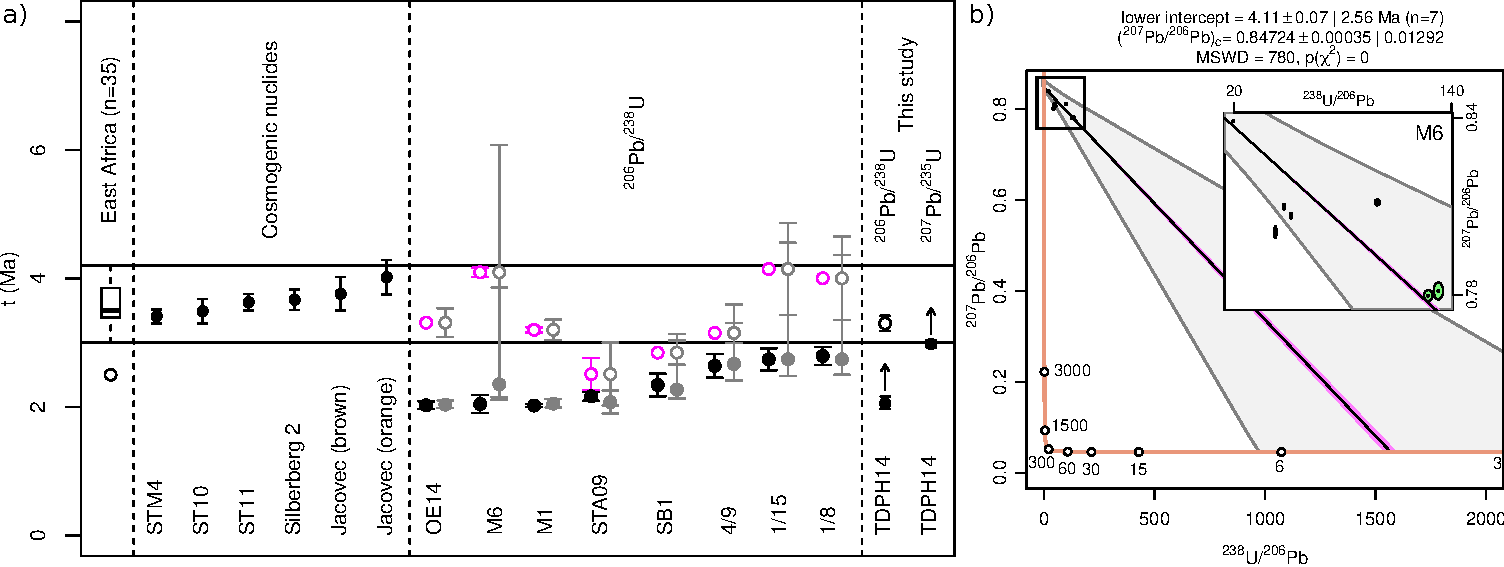
\includegraphics[width=\textwidth]{EastVsSouth2.pdf}
  \caption{a) Compilation and comparison of \emph{Australopithecus}
    chronologies for eastern Africa, shown as a box plot of hominin
    horizons \citep{maxwell2018} with \emph{Australopithecus garhi}
    from the Bouri Formation in Ethiopia as a sole outlier; and
    southern Africa. Cosmogenic nuclide ages are as reported by
    \citet{partridge2003} and \citet{granger2015,granger2022}.
    \textsuperscript{206}Pb/\textsuperscript{238}U ages (M6 and M1
    from Malapa, the rest from Sterkfontein) are from
    \citet{walker2006} and \citet{pickering2019}. STA09, SKA3 and SB1
    are from the Silberberg Grotto and may not have a stratigraphic
    association with the Sterkfontein \emph{Australopithecus} fossils
    \citep{bruxelles2019}. Empty magenta and filled black plot symbols
    mark the U--Pb dates before and after disequilibrium correction,
    respectively, with uncertainties as reported in these
    publications.  Grey symbols represent our attempt to recalculate
    these results from the original isotopic data (see panel~b).
    Sample TDPH14 yields a new age estimate for the Taung skull, as
    discussed in Section~\ref{sec:UPb-results}. The arrows indicate
    that the \textsuperscript{207}Pb/\textsuperscript{235}U isochron
    age and the disequilibrium-corrected
    \textsuperscript{206}Pb/\textsuperscript{238}U isochron age are
    minimum estimates due to post-depositional U-uptake. Note that
    other southern African samples would be likely to show U mobility
    too, if \textsuperscript{207}Pb/\textsuperscript{235}U data were
    available. b) Tera-Wasserburg diagram for sample M6, exhibiting
    extreme over-dispersion with respect to the analytical
    uncertainties. Expanding the uncertainty envelope (light grey) to
    account for this over-dispersion gives rise to the large grey
    error bars for the re-calculated U--Pb dates shown as empty grey
    symbols in panel a. The filled grey symbols and error bars of
    panel a represent the re-calculated disequilibrium corrections,
    ignoring overdispersion but assuming 2\permil{} reproducibility
    for the measured \textsuperscript{234}U/\textsuperscript{238}U
    activity ratio measurements (Section~\ref{sec:diseq}).}
  \label{fig:EastVsSouth}
\end{figure}

\section{Previous age estimates for Taung} \label{sec:review}

\subsection{Geological context}
\label{sec:geology}

There are two faunal assemblages present within the Taung Type Site:
the `Dart Deposits' (D-A to D-E) exposed by excavations at the
southern base of the Dart pinnacle \citep{mckee2016} and the
`Hrdli\v{c}ka Deposits' (H-A to H-D) exposed on the top and southern
face of the Hrdli\v{c}ka pinnacle
\citep{hrdlicka1925,mckee1994}. Based on distinct vertebrate fossil
assemblages and stratigraphic relationships, most studies recognise
the two deposits as temporally distinct, with the Dart Deposits being
older than the Hrdli\v{c}ka Deposits
\citep{mckee1994,mckee2016,frost2022}. Furthermore, the Dart Deposits
are consistently identified as the likely location of the Taung fossil
\citep{tobias1993,mckee2016,hopley2022}. Most researchers, including
Dart, have considered Taung to have been deposited within cave
sediments formed within, or contemporaneously with, the Thabaseek tufa
\citep[e.g.][]{peabody1954,tobias1993,mckee2016}. However, recent
reanalysis of the sedimentology and stratigraphy has indicated a more
complex picture of palustrine and palaeosol environments within the
Dart Deposits \citep{hopley2013,kuhn2015,parker2016} and the presence
of cave/fissure sediments and speleothems in the Hrdli\v{c}ka Deposits
\citep[][see Environments Chapter]{hopley2022}. Due to the secondary
nature of cave deposits, it is clear that the speleothems of the
Hrdli\v{c}ka Deposits are the youngest sediments of the Taung Type
Site and represent a minimum age constraint for the Taung fossil.

\subsection{Biostratigraphy}
\label{sec:biostrat}

Biostratigraphic age estimates rely on external independent sources of
chronological information, ideally well-established radiometric
ages. Prior to the first radiometric age estimates from the Cradle of
Humankind \citep{partridge2003,walker2006}, biostratigraphic
inferences relied upon faunal correlation with eastern African fossils
assemblages associated with
\textsuperscript{40}Ar/\textsuperscript{39}Ar dated volcanic
rocks. This approach was limited by the assumption that the FADs and
LADs of species or genera are shared across distinct biogeographic
regions, and because assigned ages are approximate and difficult to
verify. Using this approach \citep{mckee1993} gave the fauna from the
Taung site a biostratigraphic age estimate of 2.8--2.6\,Ma. After the
publication of U--Pb flowstone ages from multiple southern African
caves sites, \citet{pickering2019} and \citet{frost2022} were able to
use radiometric ages from within the southern African faunal province
to reduce the biogeographic uncertainties of their biostratigraphic
inferences. The similarity of the cercopithecid faunas at Taung to
those of Sterkfontein Members~2 and 4 led the authors to suggest an
age of $\sim$2.8--2.0\,Ma for Taung and $\sim$2.7--2.6\,Ma for
Makapansgat \citep{frost2022}. The validity of this approach is
dependent upon many factors, including the accuracy of the flowstone
U--Pb ages from Sterkfontein, and as we explain below there are
methodological reasons to question the accuracy of the U--Pb ages and
the biostratigraphic inferences that depend on them. In the absence of
radiometric age estimates, the age of the Taung fossil is typically
reported as $\sim$2.8\,Ma.

\subsection{Radiometric geochronology}
\label{sec:previous_geochron}

\citet{vogel1984} obtained a
\textsuperscript{234}U/\textsuperscript{238}U disequilibrium date of
$942\pm{90}$\,ka for the top of the Thabaseek formation. A follow-up
study by \citet{tobias1993} produced two more dates of
$999\pm{64}$\,ka and $762\pm{13}$\,ka, respectively.  These dates are
much younger than the biostratigraphic estimates and therefore
influence the evolutionary significance of the Taung Child. A $<1\,$Ma
age would make Taung the youngest instead of one of the oldest
specimen of \emph{Australopithecus}, far younger than the hominins
from Makapansgat, the Cradle of Humankind and eastern African
australopiths.

One way to explain the young age estimates is that Taung belongs to a
relict population of hominins who survived on the edge of the Kalahari
desert when \emph{Australopithecus} was already extinct elsewhere on
the African continent \citep{tobias1973, tobias1993,
  mckee1993}. However, the truth is likely to be more mundaine. The
Th/U disequilibrium dates are probably wrong or, more precisely, they
do not record the formation age of the Thabaseek tufa. The very high
${}^{234}$U${/}^{238}$U-activity ratios measured by \citet{vogel1984},
and the unusual variability of the dates presented by
\citet{tobias1993} likely reflect open system behaviour, whereby
uranium was added or substituted after deposition \citep{tobias1993}.
There have been no subsequent attempts to produce radiometric ages for
the Taung Type Site, instead researchers have had to settle for
biostratigraphic inference.

\section{Introduction to carbonate U--Pb geochronology}
\label{sec:UPb-method}

The U--Pb method is one of the most versatile and powerful techniques
in the geochronological toolbox. It is presently most commonly used to
date accessory minerals such as zircon, but it is increasingly applied
to other materials as well, including carbonates. The U--Pb method is
appealing in several ways. First, it does not have an upper age
limit. Whereas the Th/U disequilibrium method works best for samples
of $<500\,$ka, the U--Pb method works best for samples of $>500\,$ka.
In this sense, the U--Pb method is complementary to Th/U
disequilibrium dating.

Second, the U--Pb method contains an internal quality control
mechanism of sorts, something that is absent from most other
geochronometers. This mechanism is based on the fact that natural
uranium contains two long lived isotopes ($^{238}$U and $^{235}$U),
which decay to two different lead isotopes ($^{206}$Pb and $^{207}$Pb,
respectively).  These two decay mechanisms produce two age
estimates. If the ${}^{206}$Pb${/}^{238}$U- and
${}^{207}$Pb${/}^{235}$U-dates agree, then this gives the analyst
greater confidence the results are accurate.

Carbonate U--Pb dating is not easy.  In contrast with zircon, which
incorporates relatively high U-concentrations and low
Pb-concentrations in its crystal lattice, carbonate minerals (calcite,
dolomite, aragonite) tend to be poor in U and comparatively rich in
Pb. This `parentless' or `common' Pb has to be quantified in order to
determine the residual `radiogenic' Pb that decayed from its uranium
parent isotope, and this introduces additional uncertainty.

The common Pb problem can be solved by analysing multiple cogenetic
aliquots of the same sample, and normalising the U- and
Pb-measurements to a non-radiogenic lead isotope, ${}^{204}$Pb. This
gives rise to two coupled `isochron' equations:
\begin{equation}
  \begin{cases}
    \frac{{}^{206}\mbox{Pb}}{{}^{204}\mbox{Pb}} =
    \left[\frac{{}^{206}\mbox{Pb}}{{}^{204}\mbox{Pb}}\right]_0 +
    \left[\frac{{}^{238}\mbox{U}}{{}^{204}\mbox{Pb}}\right]\left(\exp[\lambda_{238}t]-1\right) \\
    \frac{{}^{207}\mbox{Pb}}{{}^{204}\mbox{Pb}} =
    \left[\frac{{}^{207}\mbox{Pb}}{{}^{204}\mbox{Pb}}\right]_0 +
    \left[\frac{{}^{235}\mbox{U}}{{}^{204}\mbox{Pb}}\right]\left(\exp[\lambda_{235}t]-1\right)
  \end{cases}
  \label{eq:isochron-equations}
\end{equation}

\noindent where $\lambda_{238}$ and $\lambda_{235}$ are the decay
constants of ${}^{238}$U and ${}^{235}$U, respectively; and $t$ is the
age of the sample.  Equation~\ref{eq:isochron-equations} forms two
straight lines whose intercepts correspond to the common-Pb ratios
($[^{206}\mbox{Pb}{/}^{204}\mbox{Pb}]_0$ and
$[^{207}\mbox{Pb}{/}^{204}\mbox{Pb}]_0$, respectively). In the case of
many carbonate samples, ${}^{208}$Pb can be used instead of
${}^{204}$Pb \citep{parrish2018}. This substitution is possible
because the radioactive parent of ${}^{208}$Pb is ${}^{232}$Th, which
is not generally soluble in water and therefore of very low general
abundance relative to U in carbonate.

$^{208}$Pb offers two advantages over ${}^{204}$Pb. First, it is $>30$
times more abundant, making it easier to measure and requiring shorter
mass spectrometer dwell times, thereby improving analytical
precision. Second, $^{208}$Pb is unaffected by an isobaric
interference of ${}^{204}$Hg, which makes ${}^{204}$Pb difficult to
measure by ICP-MS.

For datasets in which neither $^{204}$Pb nor $^{208}$Pb are available,
common Pb correction can also be done by plotting the
$^{207}$Pb/$^{206}$Pb-ratio against the $^{238}$U/$^{206}$Pb-ratio (a
`Tera-Wasserburg' diagram, Figure~\ref{fig:EastVsSouth}.b) and
constructing a `semitotal-Pb/U isochron' \citep{ludwig1998}.  The main
limitation of this simpler approach is that it assumes concordance of
the $^{207}$Pb/$^{235}$U and $^{206}$Pb/$^{238}$U clocks. Because the
Tera-Wasserburg diagram relies on $^{206}$Pb and $^{207}$Pb for both
deconvoluting common and radiogenic Pb, it is less able to resolve Pb
loss from common Pb heterogeneity.

\subsection{Initial disequilibrium corrections}
\label{sec:diseq}

Although Equation~\ref{eq:isochron-equations} represents two ways to
date carbonate rocks, in practice the ${}^{206}$Pb${/}^{238}$U-clock
is given far more weight than the ${}^{207}$Pb${/}^{235}$U-clock.
This is because ${}^{238}$U is $\sim$138 times more abundant than
${}^{235}$U. Consequently, $^{206}$Pb is more
abundant\footnote{$^{206}$Pb is not 138 but $<23$ times more abundant
than ${}^{207}$Pb due to the shorter half-life of ${}^{235}$U compared
to ${}^{238}$U.} and, hence, easier to measure than ${}^{207}$Pb. The
main limitation of the ${}^{206}$Pb${/}^{238}$U method -- and the
Achilles heel of carbonate U--Pb geochronology -- is the assumption of
initial secular equilibrium that underlies
Equation~\ref{eq:isochron-equations}. The problem is that ${}^{238}$U
does not decay directly to ${}^{206}$Pb, but passes by 13 short-lived
intermediate daughter `stations'. The longest-lived of these
intermediate daughters are ${}^{234}$U ($t_{1/2}=245\,$kyr) and
${}^{230}$Th ($t_{1/2}=75\,$kyr). Any initial excess or deficit of
these intermediate daughters results in an over- or under-estimated
date, respectively. Removing the resulting biases requires a
correction for any initial disequilibrium.

In the case of ${}^{230}$Th, this correction is easy.  As mentioned
before, Th is insoluble in water and is therefore generally negligible
from newly formed carbonate. It is safe to assume that these
conditions also apply to the initial concentrations of ancient
carbonates, and a simple mathematical correction can be
applied. Unfortunately, the case of ${}^{234}$U is not so
straightforward. Unlike ${}^{230}$Th, which always starts off with a
deficit relative to ${}^{238}$U, $^{234}$U can either exhibit an
initial deficit or, more commonly, an initial excess relative to
${}^{238}$U.

In some karst settings in southern Africa, the excess can reach values
up to a factor of 12 and be highly variable through time
\citep{kronfeld1994}. In fact, in Section~\ref{sec:previous_geochron}
we have already shown how parts of the Thabaseek formation are
characterised by strong ${}^{234}$U${/}^{238}$U-fractionations, which
cannot safely be assumed to remain constant through time. Applying an
initial ${}^{234}$U-correction based on an a priori estimate partly
defeats the purpose of the U--Pb method, reducing its key advantage
over Th/U disequilibrium dating.  Correcting U--Pb dates for initial
${}^{234}$U${/}^{238}$U disequilibrium requires accurate estimates of
the initial ${}^{234}$U${/}^{238}$U activity ratio. The only way to
obtain such estimates without making unverifiable assumptions is to
measure any remaining ${}^{234}$U${/}^{238}$U disequilibrium and
inferring the initial value iteratively on the assumption of a closed
system.

Accurate disequilibrium corrections are only possible for relatively
young samples. Beyond $\sim{2}\,$Ma, even the most extreme initial
${}^{234}$U${/}^{238}$U activity ratios have decayed back to a state
that is impossible to distinguish from secular equilibrium.  For
example, after 2\,Ma, an initial ${}^{234}$U${/}^{238}$U activity
ratio of 3 will be reduced to a value of 1.001782, which is only
1.7\,\permil{} above the equilibrium ratio of 1.000055
\citep[$\equiv{\lambda_{234}/[\lambda_{234}-\lambda_{238}]}$,][]{mclean2016b}. Even
if an analytical precision of 1\,\permil{} is possible, this
uncertainty balloons when extrapolating to estimate the initial ratio.

In reality, the situation is even worse because the analytical
precision of ${}^{234}$U${/}^{238}$U measurements tends to
underestimate the dispersion observed when analysing duplicate
samples. For example, \citet{walker2006} carried out ten replicate
${}^{234}$U${/}^{238}$U analyses on different aliquots of a
Sterkfontein speleothem (Figure~\ref{fig:Walker48}). With an MSWD of
2.4 and a p($\chi^2$) value of 0.01, the weighted mean of these
measurements is over-dispersed by about 20\% with respect to the
analytical uncertainties. This overdispersion corresponds to an
irreducible uncertainty of $\sim{2}$\permil{} for the
${}^{234}$U${/}^{238}$U activity ratio. The precision on a single
analysis of \textsuperscript{234}U/\textsuperscript{238}U for a locale
or specimen would risk false confidence that the measurement was
accurate and/or precise, and could lead to the illusion that the final
age is robust.

The possible bias caused by inaccurate disequilibrium corrections can
be substantial. Beyond 1.5\,Ma, the uncertainty of the disequilibrium
may exceed the correction itself. As a consequence, carbonate U--Pb
dating is subject to the same maximum age limits as Th/U
disequilibrium dating.\medskip

\begin{figure}[!ht]
  \centering
  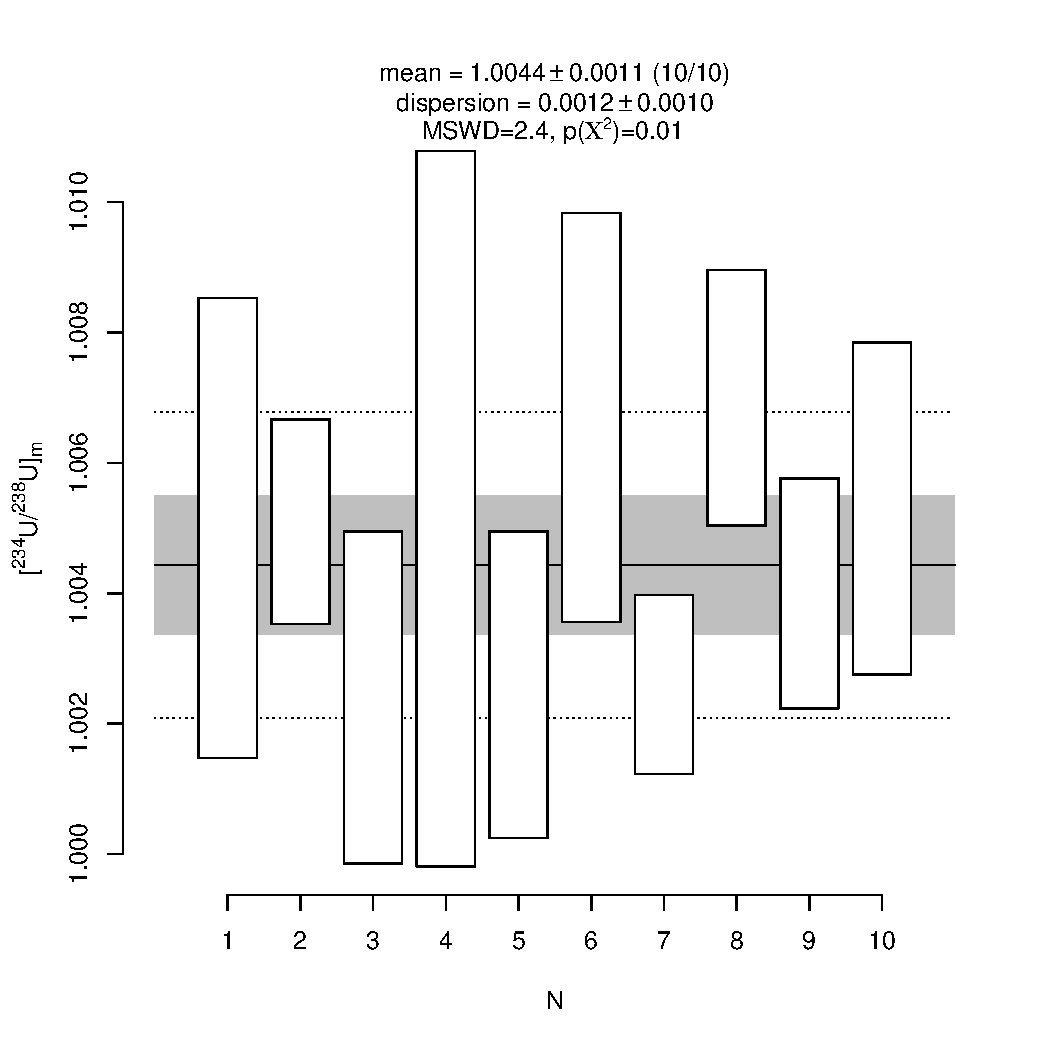
\includegraphics[width=.8\textwidth]{Walker48.pdf}
  \caption{Ten replicate $[^{234}\mbox{U/}^{238}\mbox{U}]$-activity
    ratio measurements from  \citet{walker2006}. The grey band marks
    the 95\% confidence interval for the weighted mean. The high MSWD
    and low p-value indicate that the dataset is overdispersed with
    respect to the analytical uncertainties. The overdispersion can be
    described by a random effects model with two sources of variance
    corresponding to the analytical uncertainty and the `dispersion',
    respectively  \citep{vermeesch2012c}. The dotted line marks the
    95\% confidence interval corresponding to the dispersion. For the
     \citet{walker2006} dataset, it is about 2\permil{} wide.}
  \label{fig:Walker48}
\end{figure}

\subsection{A critical appraisal of existing U--Pb dates for southern
African hominin sites}
\label{sec:appraisal}

Figure~\ref{fig:sensitivity} presents a selection of 31 published
carbonate U--Pb data from southern African hominin discovery sites,
including the landmark study of \citet{walker2006}, the Malapa data of
\citet{dirks2010} and the 26-sample compilation of
\citet{pickering2019}. The new Taung data from
Section~\ref{sec:UPb-results} are also shown for comparison.

The figure consists of two parts. Panel a) shows the magnitude of the
disequilibrium correction.  Panel b) shows its precision.  Solid lines
represent different initial ${}^{234}$U${/}^{238}$U-activity
ratios. The initial ${}^{230}$Th${/}^{238}$U-activity ratio was
assumed to be zero ($[^{230}$Th${/}^{238}$U$]_i=0$) in all
cases.

The magnitude of the disequilibrium correction (panel a) was
calculated as follows:

\begin{enumerate}
\item Given the initial ${}^{234}$U${/}^{238}$U-activity ratio and the
  disequilibrium-corrected U--Pb age ($t_c$), predict the present-day
  ${}^{206}$Pb${/}^{238}$U-ratio.
\item Use this ${}^{206}$Pb${/}^{238}$U-ratio to calculate the
  uncorrected (`raw') ${}^{206}$Pb${/}^{238}$U-date ($t_r$).
\item Define the relative magnitude of the disequilibrium correction
  as $(t_r-t_c)/t_c$. Note that this is an `optimistic' way to
  quantify the size of the correction.  Using the corrected age in the
  numerator would produce larger values.
\end{enumerate}

Panel a) relates to the accuracy of the disequilibrium correction: the
greater the correction, the more likely it is to be inaccurate. In
contrast, panel b) visualises the precision of the correction. This is
calculated as follows:

\begin{enumerate}
\item\label{it:pred} Use the initial ${}^{234}$U${/}^{238}$U-activity
  ratio ($[^{234}$U${/}^{238}$U$]_i$) to predict the present-day
  ${}^{234}$U${/}^{238}$U-activity ratio
  ($[^{234}$U${/}^{238}$U$]_m$) and the present-day
  ${}^{206}$Pb${/}^{238}$U ratio.
\item Add/subtract 2\permil{} uncertainty to/from
  $[^{234}$U${/}^{238}$U$]_m$ to obtain two limits
  $[^{234}$U${/}^{238}$U$]_u$ and $[^{234}$U${/}^{238}$U$]_l$,
  respectively. Note that this calculation ignores the overdispersion
  issues highlighted in Figure~\ref{fig:EastVsSouth} and, therefore,
  paints an optimistic picture of the situation.
\item Combine $[^{234}$U${/}^{238}$U$]_u$ and
  $[^{234}$U${/}^{238}$U$]_l$ with the predicted
  ${}^{206}$Pb${/}^{238}$U-ratio from step~\ref{it:pred} to obtain two
  age limits $t_l$ and $t_u$.
\item Define the relative precision as $(t_u-t_l)/t_c$.
\end{enumerate}

The solid lines of Figure~\ref{fig:sensitivity}b terminate where it is
no longer possible to obtain a physically-plausible solution. This can
either happen when $[^{234}$U${/}^{238}$U$]_l<1.000055$ and $t$ is
sufficiently high so that $[^{234}$U${/}^{238}$U$]_i=0$; or when
$[^{234}$U${/}^{238}$U$]_l>1.000055$ and $t$ is sufficiently high so
that $[^{234}$U${/}^{238}$U$]_i>20$.

The dashed line in Figure~\ref{fig:sensitivity}.b marks the
uncertainty envelope for ${}^{206}$Pb${/}^{238}$U dates that lack
initial disequilibrium constraints, either because
${}^{206}$Pb${/}^{238}$U was not measured or because the
disequilibrium has expired. This envelope was calculated as the
difference between the ${}^{206}$Pb${/}^{238}$U-date with an initial
${}^{234}$U${/}^{238}$U-activity ratio $[^{234}$U${/}^{238}$U$]_i=12$
\citep[the highest value reported by][]{kronfeld1994} and
$[^{206}$Pb${/}^{238}$U$]_i=1$ (no initial uranium disequilibrium).

In absolute terms, $\Delta{t}$ increases from 0\,Myr at $t=0$ to
3.9\,Myr at $t=\infty$, but in relative terms, the uncertainty
decreases from $\Delta{t}/t=\infty$ at $t=0$ to $\Delta{t}/t=0$ at
$t=\infty$. At the 2--4\,Ma timescales of interest, the unconstrained
${}^{206}$Pb${/}^{238}$U age uncertainty hovers around 80--90\%. This
large uncertainty is the reason why it is so important to apply a
disequilibrium correction to carbonate ${}^{206}$Pb${/}^{238}$U-dates
in the first place, particularly in areas of high
$[^{234}$U${/}^{238}$U$]_i$ variability such as the Cradle of
Humankind.

For sufficiently old samples, the uncertainty of the disequilibrium
correction (i.e., $t_u-t_l$) may exceed the correction itself
($t_r-t_c$). For initial $^{234}$U${/}^{238}$U activity ratios of 1, 2
and 4 (assuming $[^{230}$Th${/}^{238}$U$]_i=0$), this occurs for ages
exceeding 1.54, 2.04 and 2.58\,Ma, respectively.

Thirty-two U--Pb measurements are shown as circles in
Figure~\ref{fig:sensitivity}. Half of them are associated with
disequilibrium corrections exceeding 30\% of the uncorrected age
(corresponding to 43\% of the corrected age), and uncertainties of
greater than 10\%. Four samples fall in the `forbidden zone' with
unresolvable $[^{234}$U${/}^{238}$U$]_i$-values. It is also useful to
observe that the oldest samples tend to have the highest inferred
$[^{234}$U${/}^{238}$U$]_i$-values. This is likely a numerical
artifact caused by extrapolation of a very small amount of residual
disequilibrium and/or open system behaviour with addition or
replacement of initial U with U with more marked disequilibrium.

In summary, Figure~\ref{fig:sensitivity} casts doubt on the value of
disequilibrium-corrected carbonate ${}^{206}$Pb${/}^{238}$U dates.
Fortunately, there is a solution to the ${}^{234}$U${/}^{238}$U
disequilibrium conundrum. For old samples, the complications of the
${}^{234}$U/${}^{238}$U disequilibrium correction can be circumvented
by avoiding the ${}^{206}$Pb${/}^{238}$U-method altogether, and using
the ${}^{207}$U${/}^{235}$U-method instead.  This will be explained in
the next section.\medskip

\begin{figure}[!ht]
  \centering
  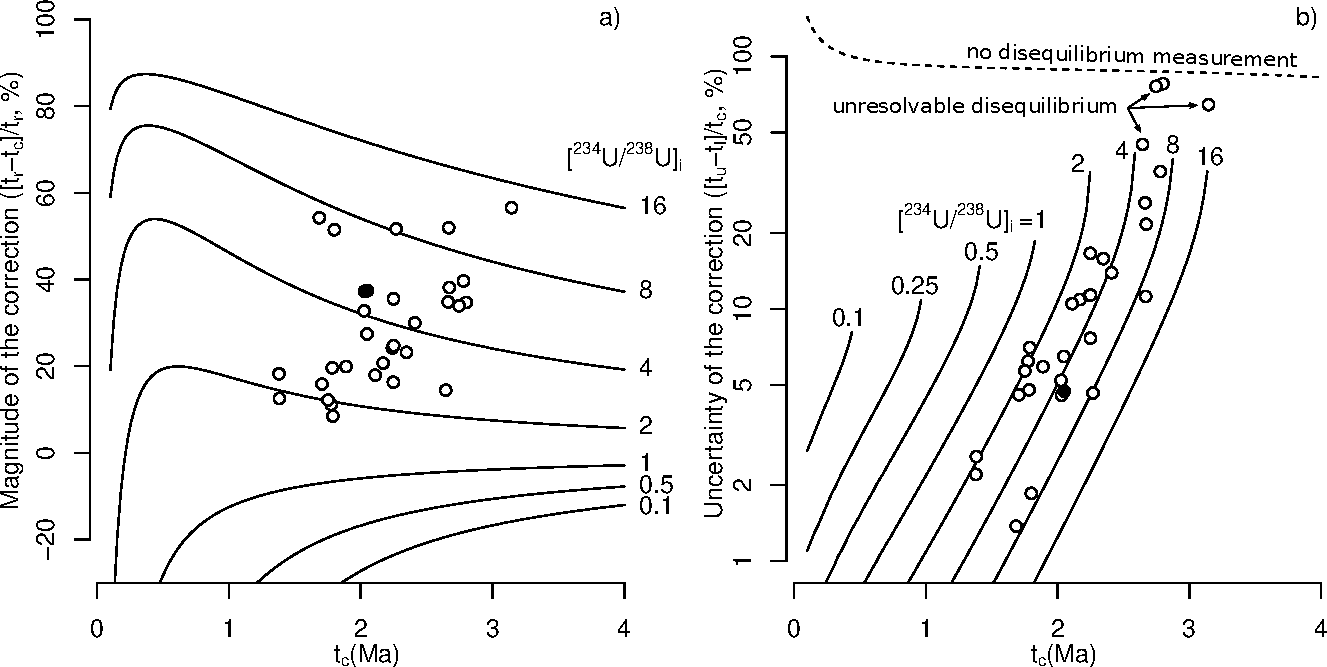
\includegraphics[width=\textwidth]{CradleAccuracyPrecision.pdf}
  \caption{Relative magnitude (a) and precision (b) of the initial
    ${}^{234}$U${/}^{238}$U disequilibrium correction against the
    corrected carbonate ${}^{206}$Pb${/}^{238}$U date ($t_c$), for
    different values of the initial ${}^{234}$U${/}^{238}$U activity
    ratio (solid lines).  The dashed line in panel b) marks the
    relative uncertainty interval when no disequilibrium measurement
    is available, defined as the difference between corrected dates
    using assumed initial ${}^{234}$U${/}^{238}$U activity ratios of 1
    and 12. Empty circles mark 31 published U--Pb dates from
    \citet{walker2006}, \citet{dirks2010} and \citet{pickering2019}
    listed in Table~\ref{tab:sensitivity}. The black circles mark the
    new U--Pb date for Taung sample TDPH14
    (Section~\ref{sec:UPb-results}).  Panel~a) shows that this sample
    has a disequilibrium-corrected U-Pb date ($t_c$) of 2.05\,Ma,
    which is 40\% younger than the uncorrected date ($t_r$). This age
    difference is caused by an iteratively calculated initial
    ${}^{234}$U${/}^{238}$U-activity ratio of 4.9.  Assuming a
    reproducibility of the present-day ${}^{234}$U${/}^{238}$U
    measurement of 2\permil, panel~b) shows that the disequilibrium
    correction has an analytical precision of 5\%. The four published
    datasets marked by the arrows in panel b) have measured
    ${}^{234}$U${/}^{238}$U activity ratios that are within {2\permil}
    of secular equilibrium.}
  \label{fig:sensitivity}
\end{figure}

\subsection{The ${}^{207}$Pb${/}^{235}$U method}\label{sec:Pb207U235}

Even though the ${}^{207}$Pb${/}^{235}$U clock is less precise than
the (uncorrected) ${}^{206}$Pb${/}^{238}$U clock, it can be precise
enough for samples that are reasonably old and relatively rich in
uranium. Crucially, the loss of precision is compensated by a gain in
accuracy \citep{richards1998,vaks2020,engel2019}.

Whereas the ${}^{238}$U decay series contains two long-lived
intermediate daughters, the ${}^{235}$U series contains only one such
daughter, $^{231}$Pa ($t_{1/2}=32.7\,$kyr). This nuclide is easy to
deal with because Pa is chemically similar to Th. Therefore,
$^{231}$Pa is always depleted in newly formed carbonates, so that its
initial activity ratio can be safely neglected.  Even if the
assumption of zero ${}^{231}$Pa is wrong, the consequences of this
wrong assumption are small. This is because, unlike the ${}^{234}$U
correction, which can range from $-17\%$ to $>+100\%$, the
${}^{231}$Pa correction only ranges from $-2\%$ to $0\%$ (assuming a
true age of 2\,Ma). There are two reasons why the southern African
carbonate U--Pb datasets of \citet{pickering2019}, \citet{dirks2010}
and \citet{walker2006} cannot be re-evaluated using the
${}^{207}$Pb${/}^{235}$U method.

First, the data tables provided in these publications are formatted in
terms of ${}^{238}$U${/}^{206}$Pb, ${}^{207}$Pb${/}^{206}$Pb and
${}^{204}$Pb${/}^{206}$Pb ratios.  In principle, it is possible to
compute the ${}^{207}$Pb${/}^{235}$U ratio from the
${}^{238}$U${/}^{206}$Pb and ${}^{207}$Pb${/}^{206}$Pb ratios,
provided that the error correlation between all the ratios are
provided. Unfortunately, most of these error correlations are either
not provided with the published southern African flowstone U--Pb
datasets, or they are suspect due to the presence of physically
impossible values ($<-1$ or $>1$). This is why
Figure~\ref{fig:EastVsSouth}.b assumes zero error correlations (error
ellipses parellel to the plot axes).

Second, many of these published studies do not provide information on
${}^{208}$Pb. This is unfortunate because ${}^{208}$Pb can be measured
more precisely than ${}^{204}$Pb, which is important to compensate for
the lower precision of the ${}^{207}$Pb${/}^{235}$U ratio
measurements. Fortunately, some studies do include ${}^{208}$Pb
ratios, including those of \citet{walker2005} and
\citet{walker2006}. Figure~\ref{fig:Makapansgat} shows an unpublished
ID-TIMS dataset from a lone sample (LAB03) of the Makapansgat
Limeworks presented by \citet{walker2005}. Neither the dataset of
\citet{walker2005} nor that of \citet{walker2006} provides all the
error correlations needed to fully propagate the uncertainties of the
isochron ratios.

The LAB03 sample is a piece of Member~1b flowstone collected from the
area between the Original Ancient Entrance (OAE) and the North Alcove
of the Main Quarry \citep{walker2005,reed2022}. The flowstone was
deposited prior to the in-filling of the cave with clastic sediments,
so is older than all the fossil-bearing units of the Makapansgat
Limeworks: Members~2--5 and Rodent Corner
\citep{maguire1984,reed2022}. Unfortunately, it is not currently
possible to determine the time that elapsed between the deposition of
Member~1b flowstone and the overlying sedimentary units. Most of the
\emph{Australopithecus} fossils were collected \emph{ex situ} from
lime dumps and have been confidently assigned to Member~3; therefore,
LAB03 provides a maximum age estimate for all fossils including
\emph{Australopithecus africanus} from the Makapansgat Limeworks.

With this caveat in mind, Figure~\ref{fig:Makapansgat} conveys several
important pieces of information. First, the LAB03 sample is old
($>4.4$\,Ma using the 95\% confidence interval for the
${}^{207}$Pb/$^{235}$U isochron age as a lower bound). This antiquity
is consistent with biostratigraphic evidence for Makapansgat Member 3
being among the oldest fossil assemblages in southern Africa
\citep{mckee1993,frost2022} and with magnetostratigraphic inference
for the OAE flowstones belonging to the Gilbert magnetochron at
approximately 4\,Ma \citep{hopley2007}. The age of LAB03 is also
comparable with the $4.9 \pm 1.9$\,Ma ${}^{207}$Pb/$^{235}$U isochron
age for the Hoogland Basal Speleothem \citep{hopley2019}, suggesting
that Mio-Pliocene age flowstones may be a common feature of southern
African palaeo-karst. Second, there is a significant difference
between the ${}^{206}$Pb/$^{238}$U and ${}^{207}$Pb/$^{235}$U isochron
ages (7.92 and 5.28\,Ma, respectively). Third, the
${}^{207}$Pb/$^{235}$U date is less precise than the
${}^{206}$Pb/$^{238}$U date, with 95\% confidence intervals of 0.11
and 0.87\,Ma wide, respectively.

The significant difference between the two types of U--Pb dates for
LAB03 is likely the result of initial ${}^{234}$U/${}^{238}$U
disequilibrium. Due to its old age, it is not possible to undo the
effects of this disequilibrium. However, we do know that the effect of
\textsuperscript{234}U/\textsuperscript{238}U disequilibrium on
${}^{206}$Pb/$^{238}$U isochrons can exceed $1$\,Ma, whereas the
effect of \textsuperscript{231}Pa/\textsuperscript{235}U
disequilibrium is capped at 30\,ka
(Section~\ref{sec:Pb207U235}). Therefore, we conclude that the
${}^{207}$Pb/$^{235}$U isochron is more accurate than the
${}^{206}$Pb/$^{238}$U isochron, amply compensating for its lesser
precision.

Having illustrated the ${}^{207}$Pb${/}^{235}$U method, we reiterate
that the results shown in Figure~\ref{fig:Makapansgat} are negatively
affected by the absence of a full covariance structure. Knowledge of
all error correlations would improve the precision of the estimated
isochron age.  In order to take full advantage of the
${}^{207}$Pb/${}^{235}$U method, it is necessary to either reprocess
the raw mass spectrometer data from the published studies that report
${}^{204}$Pb and/or ${}^{208}$Pb, or to start over again and
re-analyse all the hominin discovery sites. The next section will
start this effort with some new ${}^{207}$Pb${/}^{235}$U dates, which
we believe to serve as a robust minimum age constraint for
Taung.\medskip

\begin{figure}[!ht]
  \centering
  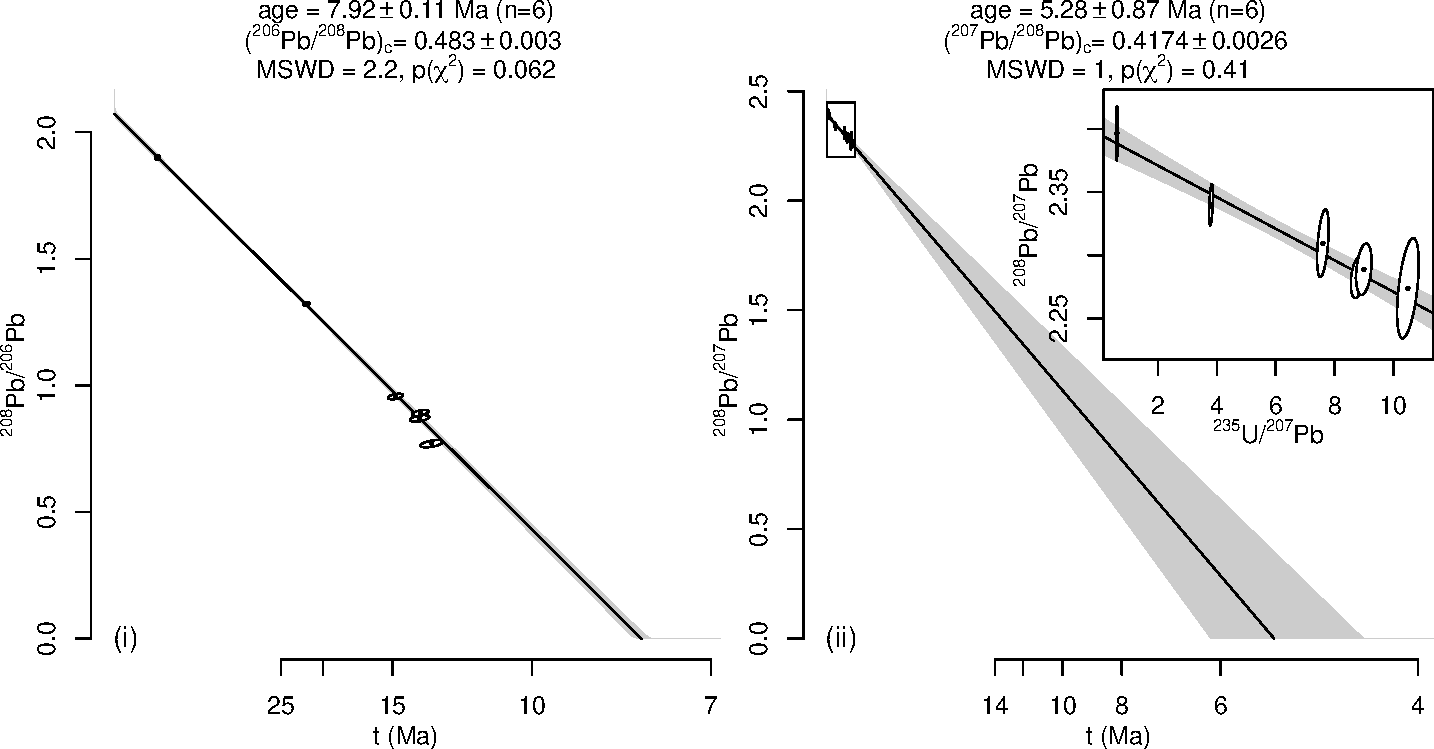
\includegraphics[width=\textwidth]{Makapansgat.pdf}
  \caption{TIMS U--Pb data for Makapansgat Limeworks sample LAB03 of
    \citet{walker2005}, presented as (i)
    \textsuperscript{206}Pb/\textsuperscript{238}U and (ii)
    \textsuperscript{207}Pb/\textsuperscript{235}U inverse isochrons
    \citep{li2021}. The former is more precise but less accurate than
    the latter, due to the inability to correct for initial
    disequilibrium beyond 2\,Ma. Error correlations for these inverse
    isochron plots were calculated from the conventional isochron
    ratios reported in the data source, which were assumed to be
    uncorrelated.  This assumption is likely incorrect, which has a
    minor effect on the isochron age and a major effect on its
    uncertainty, which is therefore wrong. Note that knowledge of the
    error correlations would reduce the uncertainty of the fit.}
  \label{fig:Makapansgat}
\end{figure}

\section{New U--Pb age constraints for Taung}
\label{sec:UPb-results}

During the 2010 field season at the Taung site, a number of carbonate
samples (speleothems and tufas) were collected from the Dart pinnacle,
the Hrdli\v{c}ka pinnacle, and the intervening deposits exposed in the
quarry floor of the disused Buxton-Norlim limeworks.  The samples were
screened by LA-ICP-MS to assess their suitability for U--Pb
dating. Suitable samples exhibit relatively high U-concentrations and
a wide range of Pb/U-ratios providing the potential to form a well
defined isochron line. Only one sample fulfilled all these criteria.

TDPH14 is a flowstone that was collected near the top of the
Hrdli\v{c}ka pinnacle at an altitude of 1150\,m a.s.l. (see
Figure~\ref{fig:TDPH14ICPMS}.i and the Environments Chapter for
further details). The sample is a steeply-dipping brown and white
flowstone, approximately 10\,cm thick and composed of both aragonite
and calcite. Its position high in the stratigraphic sequence, and its
cavity-filling nature, offer a minimum age for both the Taung Type
Site and the Taung skull.

The sample was cut, polished and subjected to a preliminary isotopic
analysis along an LA-ICP-MS transect
(Figure~\ref{fig:TDPH14ICPMS}.ii).  This screening revealed
significant variability in U-concentration across the flowstone's
laminations, with values ranging from 1\,ppb to 35\,ppm
(Figure~\ref{fig:TDPH14ICPMS}.iii). Targeting the most radiogenic
layers of the sample yields a ${}^{206}$Pb/${}^{238}$U date of
$3.166\pm{0.065}$\,Ma (Figure~\ref{fig:TDPH14ICPMS}.v). This falls
well outside the detectable range for ${}^{234}$U/${}^{238}$U
disequilibrium, casting doubt on the accuracy of the LA-ICP-MS
data. Unfortunately, ${}^{207}$Pb and ${}^{208}$Pb signals were too
low to construct a sufficiently precise ${}^{207}$Pb/${}^{235}$U
isochron. A more precise ID-TIMS analysis of four aliquots of TDPH was
undertaken to remediate this issue.\medskip

\begin{figure}[!ht]
  \centering
  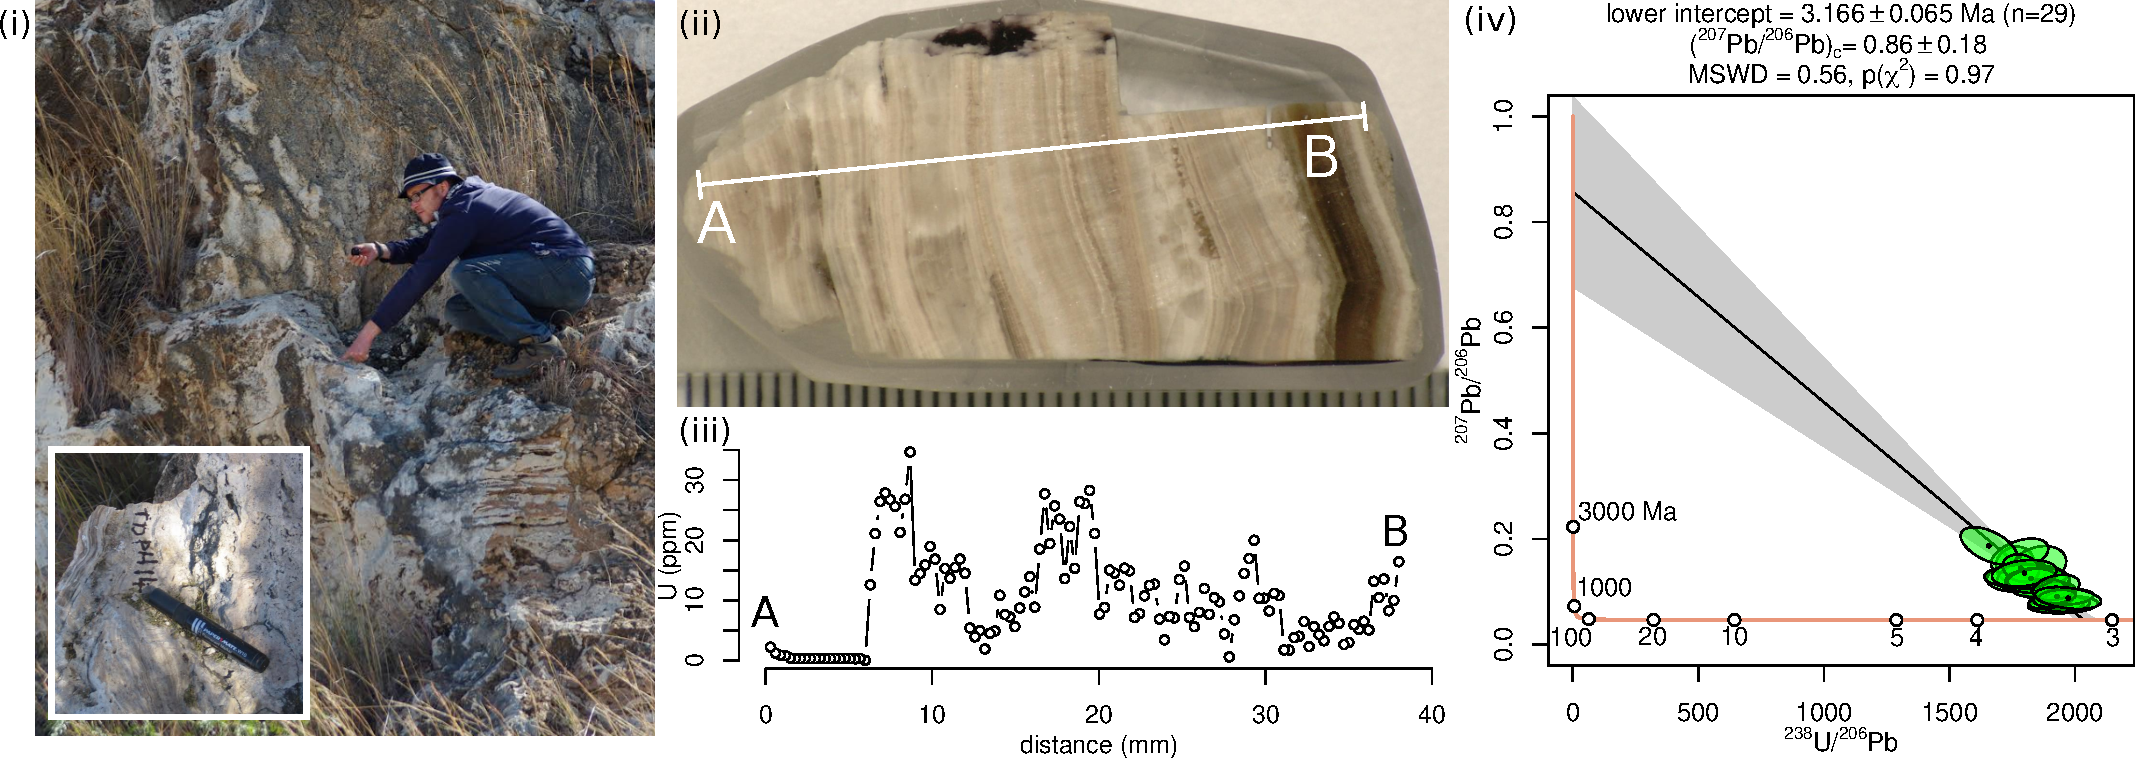
\includegraphics[width=\linewidth]{TDPH14ICPMS2.pdf}
  \caption{LA-ICP-MS data for sample TDPH14. (i) Field photograph of
    the sample location; (ii) a polished hand specimen of the sample;
    (iii) uranium concentration along the profile shown in the
    previous panel; (iv) semitotal-Pb/U isochron from a targeted
    high-U zone. The ${}^{238}$U--${}^{206}$Pb ratios are not
    corrected for initial disequilibrium.}
  \label{fig:TDPH14ICPMS}
\end{figure}

Four aliquots of TDPH14 yield an uncorrected ${}^{206}$Pb/${}^{238}$U
`errorchron' age of $3.30\pm{0.12}$\,Ma (MSWD=49), which agrees with
the LA-ICP-MS age (Figure~\ref{fig:TIMS}.ii). Isotope dilution ICP-MS
analysis of the sample indicates a present-day ${}^{234}$U/${}^{238}$U
activity ratio of $1.0117\pm{0.0059}$ (Figure~\ref{fig:TIMS}.iii). The
${}^{234}$U/${}^{238}$U activity ratio measurements are over-dispersed
with respect to the analytical uncertainties. Due to the small number
of aliquots (i.e., four), it is not possible to identify `outliers' or
to quantify the over-dispersion. Taking the weighted mean
${}^{234}$U/${}^{238}$U ratio at face value and using it to correct
the ${}^{206}$Pb/${}^{238}$U isochron for initial disequilibrium
changes the date from $3.30\pm{0.12}$ to $2.05+0.11/-0.08$\,Ma.  This
40\% reduction in age implies an initial ${}^{234}$U/${}^{238}$U
activity ratio of 4.9 (Figure~\ref{fig:TIMS}.iv).

Switching to ${}^{207}$Pb/${}^{235}$U space yields a well defined
isochron of $2.982\pm{0.057}$\,Ma (assuming no initial
${}^{231}$Pa). This is similar to the uncorrected
${}^{206}$Pb/${}^{238}$U isochron age, implying that the sample was
close to secular ${}^{234}$U/${}^{238}$U equilibrium at the time of
formation. The ${}^{207}$Pb/${}^{235}$U isochron is more precise than
the disequilibrium-corrected ${}^{206}$Pb/${}^{238}$U isochron. It is
also less dispersed with an MSWD of 0.7 as opposed to value of 49 for
the ${}^{206}$Pb/${}^{238}$U isochron. The two isochron age estimates
do not overlap within the analytical uncertainties. This disagreement
may be caused by open system behaviour of uranium, similar to that
which was reported by \citet{tobias1993} for the Th/U data of
\citet{vogel1984} and \citet{tobias1993}. Recent changes in
${}^{234}$U/${}^{238}$U activity ratios would result in an
over-estimated ${}^{234}$U/${}^{238}$U-disequilibrium correction and,
hence, an under-estimated ${}^{206}$Pb/${}^{238}$U isochron age. It
would have a similar but smaller effect on the
${}^{207}$Pb/${}^{235}$U age. It is possible that the lower MSWD of
the ${}^{207}$Pb/${}^{235}$U isochron reflects the smaller degree of
isotopic disturbance.

Assuming uranium is only gained and not lost over time, both the
disequilibrium-corrected ${}^{206}$Pb/${}^{238}$U and
${}^{207}$Pb/${}^{235}$U isochron ages are minimum age
estimates. Consequently, the oldest date is the most useful one.
Hence, we use the ${}^{207}$Pb/${}^{235}$U age to constrain the age of
TDPH14.  Given its location at the top of the Hrdli\v{c}ka pinnacle,
and following \citet{hopley2013}'s interpretation that the
hominin-bearing unit was laid down in stratigraphic succession with
the surrounding tufa deposits, the new flowstone date provides a lower
age limit for the Taung skull. In order to obtain a potential upper
age bracket for the fossil, a second sample is needed from below the
PCS horizon. To this end, two boreholes were drilled in 2012 (see
Environments Chapter), one in the Dart pinnacle (13.7\,m) and one in
the Hrdli\v{c}ka pinnacle (48.5\,m). Unfortunately, LA-ICP-MS
screening of neither core yielded any suitable material for U--Pb
dating. The search for an upper age limit continues.\medskip

\begin{figure}[!ht]
  \centering
  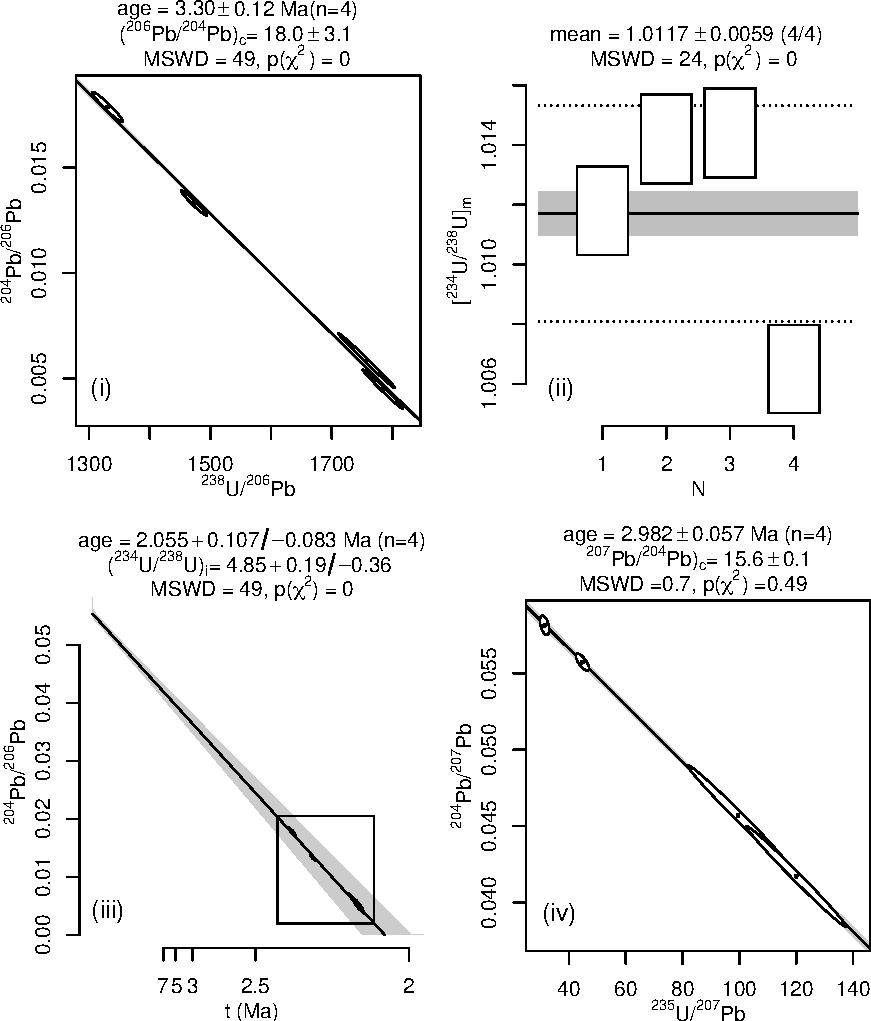
\includegraphics[width=.8\textwidth]{TIMS.pdf}
  \caption{TIMS U--Pb data for sample TDPH14, shown as inverse
    isochrons. (i) uncorrected ${}^{238}$U--${}^{206}$Pb isochron;
    (ii) measured ${}^{234}$U/${}^{238}$U-activity ratios; (iii)
    disequilibrium-corrected ${}^{238}$U--${}^{206}$Pb isochron with a
    box showing the outline of panel i; (iiv)
    ${}^{235}$U--${}^{207}$Pb isochron. Data are reported in
    Table~\ref{tab:TIMS}.}
  \label{fig:TIMS}
\end{figure}

\section{Conclusion}

Since its discovery a century ago, Taung has challenged
scientists. With the fossil itself being just a partially preserved
juvenile skull, it took nearly two decades before most
palaeoanthropologists agreed it was a human ancestor
\citep{keith1947}. This helped settle the debate between proponents of
Asia and Africa being the origin of the hominin clade.

The age of Taung, and of other early southern African hominins,
remains poorly constrained, and this contribution has summarised just
a subset of the numerous attempts to resolve this issue. In addition
to the biostratigraphic and isotopic methods discussed above,
archaeologists have applied numerous other dating techniques to the
southern African hominin sites, including electron spin resonance
dating, palaeomagnetic surveys, optically and thermally stimulated
luminescence dating, and even U--Th--He thermochronology
\citep{schwarcz1994, herries2011, pickering2013, makhubela2022}.

With so many inconsistent dates to choose from, there is a risk that
palaeoanthropologists will pick the dates that best suit their
preconceived ideas about human evolution. This potentially leads to
circular reasoning and impedes scientific progress. Better and more
consistent absolute dating methods are needed to break out of this
cycle. The challenges posed by the southern African australopiths in
general, and by Taung in particular, are an important driving force
for methodological developments in radiometic geochronology.

The advent, nearly 20 years ago, of carbonate U--Pb geochronology,
promised to be the much sought after breakthrough \citep{walker2006}.
Disequilibrium-corrected
\textsuperscript{206}Pb/\textsuperscript{238}U isochron dates were
subsequently determined on dozens of southern African flowstones, most
of which are summarised in Figure~\ref{fig:sensitivity}. The results
of these studies suggest that the southern African hominins were
substantially younger than their eastern African counterparts, and
some researchers have drawn detailed environmental conclusions from
these dates \citep{pickering2019}. However, given the importance of
the research questions at hand, it is important to remain vigilant and
self-critical.

The disagreement between the U--Pb dates and independently-determined
cosmogenic nuclide dates at Sterkfontein raises questions about the
geological significance of these results
\citep{granger2015,kramers2017,granger2022}. The quantitative analysis
presented in this contribution reveals that the analytical uncertainty
of several disequilibrium-corrected
\textsuperscript{206}Pb/\textsuperscript{238}U isochron dates has been
under-estimated by hundreds of thousands of years, and in some cases
more than a million years.

We advocate the use of the
\textsuperscript{207}Pb/\textsuperscript{235}U isochron method as a
more accurate alternative. Our proposal simplifies a suggestion by
\citet{engel2019}, who point out that the ${}^{207}$Pb/${}^{235}$U age
should be concordant with the ${}^{206}$Pb/${}^{238}$U age, and that
this concordance could be used to back-calculate the initial
${}^{234}$U/${}^{238}$U ratio in cases where reliable
${}^{234}$U/${}^{238}$U measurements are not possible.
\citet{engel2019} suggest using this inferred activity ratio to obtain
a disequilibrium-corrected ${}^{206}$Pb/${}^{238}$U date.  We argue
that if the ${}^{207}$Pb/${}^{235}$U and ${}^{206}$Pb/${}^{238}$U ages
are incompatible, then the ${}^{207}$Pb/${}^{235}$U age is far more
likely to be correct, and should be taken as the best estimate of the
true age.  Beyond 2\,Ma (and, in some cases, before that), all the
age-resolving power of the paired ${}^{206}$Pb/${}^{238}$U and
${}^{207}$Pb/${}^{235}$U approach resides in the
${}^{207}$Pb/${}^{235}$U clock, so the ${}^{206}$Pb/${}^{238}$U data
add no value.

Although we did not manage to obtain a definitive age estimate for the
Taung skull in time for the centenary celebration of its discovery, we
did make some meaningful progress towards this goal. We used the
\textsuperscript{207}Pb/\textsuperscript{235}U method to provide a
tentative $\sim{5.28}$\,Ma upper age limit for the Makapansgat
Limeworks deposit, which has been biostratigraphically linked to Taung
\citep{mckee1993}. We also obtained a minimum age estimate of
$2.98\pm{0.06}$\,Ma for the Taung skull.

These preliminary results open the prospect of future progress.  Our
\textsuperscript{207}Pb/\textsuperscript{235}U isochron age is closer
to the uncorrected \textsuperscript{206}Pb/\textsuperscript{238}U age
than it is to the disequilibrium-corrected
\textsuperscript{206}Pb/\textsuperscript{238}U age. Naively assuming
that the same phenomenon applies to other hominin discovery sites
would resolve the discrepancy between the cosmogenic nuclide and U--Pb
dates shown in Figure~\ref{fig:EastVsSouth}.

It would be premature to claim success. A lot more work is needed and
it is unlikely that the \textsuperscript{207}Pb/\textsuperscript{235}U
method is the panacea for all of the problems linked to dating the
southern African australopiths. One issue is that post-depositional
uranium uptake remains a challenge. Although the
\textsuperscript{207}Pb/\textsuperscript{235}U method is less affected
by it than the \textsuperscript{206}Pb/\textsuperscript{238}U and Th/U
methods, it is not immune.

The debate about the relevance of the Taung skull was concluded when
once vocal opponents of Raymond Dart's hypothesis graciously admitted
that they had been wrong \citep{keith1947}. Geochronologists,
including the authors of this contribution, would do well to have a
similar attitude.  If there is one thing that can be learned from
100~years of research into Taung, then it is that scientific progress
is not always linear. The solution of the riddle of human evolution
will require humility and a lot of patience.\medskip

\begin{table}[!ht]
  \begin{tabular}{llllll}
    \hline
    paper & site & sample & age &
    $\left[^{234}\mbox{U}{/}^{238}\mbox{U}\right]_i$ &
    $\left[^{234}\mbox{U}{/}^{238}\mbox{U}\right]_m$ \\ \hline
    \citet{walker2006} & Sterkfontein & STA09 & 2.17 & 2.92* & 1.0043 \\
    \citet{walker2006} & Sterkfontein & STA12 & 2.11 & 2.62* & 1.0043 \\
    \citet{walker2006} & Sterkfontein & STA15 & 2.24 & 3.34* & 1.0043 \\
    \citet{walker2006} & Sterkfontein & SKA3 & 2.25 & 3.41* & 1.0043 \\
    \citet{dirks2010} & Malapa & NHL09 & 2.026 & 4.12* & 1.0103 \\
    \citet{pickering2019} & Coopers’s cave & CD-1 & 1.38 & 2.22 & 1.0248 \\
    \citet{pickering2019} & Bolt’s farm & WP-160-1 & 2.78 & 6.48* & 1.0022 \\
    \citet{pickering2019} & Bolt’s farm & WP-160-2 & 2.269 & 8.186 & 1.0119 \\
    \citet{pickering2019} & Bolt’s farm & BFMC-1 & 1.776 & 1.95* & 1.0064 \\
    \citet{pickering2019} & Bolt’s farm & BFMC-6 & 1.383 & 1.901 & 1.0182 \\
    \citet{pickering2019} & Bolt’s farm & AV01 & 2.41 & 4.232 & 1.0036 \\
    \citet{pickering2019} & Bolt’s farm & AV03 & 2.668 & 9.46* & 1.0046 \\
    \citet{pickering2019} & Bolt’s farm & WP-160-6L & 1.752 & 2.011 & 1.0072 \\
    \citet{pickering2019} & Drimolen & DN26 & 1.889 & 2.652 & 1.0078 \\
    \citet{pickering2019} & Drimolen & DN09 & 1.789 & 1.789 & 1.0050 \\
    \citet{pickering2019} & Drimolen & DN39-A & 2.673 & 5.971 & 1.0025 \\
    \citet{pickering2019} & Drimolen & DMK5 & 2.664 & 5.336 & 1.0023 \\
    \citet{pickering2019} & Haasgat & HG1 & 1.686 & 7.03 & 1.0508 \\
    \citet{pickering2019} & Hoogland & HL1 & 3.145 & 12.879 & 1.0016 \\
    \citet{pickering2019} & Malapa & M6 & 2.048 & 3.51 & 1.0065 \\
    \citet{pickering2019} & Malapa & M1\_1 & 2.026 & 4.11* & 1.0103 \\
    \citet{pickering2019} & Sterkfontein & OE14 & 2.03 & 4.739 & 1.0119 \\
    \citet{pickering2019} & Sterkfontein & OE13 & 1.784 & 2.558 & 1.0099 \\
    \citet{pickering2019} & Sterkfontein & 1/8 & 2.8 & 5.515 & 1.0016 \\
    \citet{pickering2019} & Sterkfontein & 4/9 & 2.645 & 2.578 & 1.0009 \\
    \citet{pickering2019} & Sterkfontein & 1/15 & 2.747 & 5.301 & 1.0018 \\
    \citet{pickering2019} & Sterkfontein & SB1 & 2.347 & 3.32 & 1.0031 \\
    \citet{pickering2019} & Swartkrans & SWK-5 & 1.8 & 6.756 & 1.0352 \\
    \citet{pickering2019} & Swartkrans & SWK-7 & 2.248 & 2.555 & 1.0027 \\
    \citet{pickering2019} & Swartkrans & SWK-9 & 1.706 & 2.237 & 1.0098 \\
    \citet{pickering2019} & Swartkrans & SWK-12 & 2.249 & 4.824 & 1.0065 \\
    \hline
  \end{tabular}
  \caption{The underlying data for
    Figure~\ref{fig:sensitivity}. Asterisks mark
    $\left[^{234}\mbox{U}{/}^{238}\mbox{U}\right]_i$-values inferred
    from the
    $\left[^{234}\mbox{U}{/}^{238}\mbox{U}\right]_m$-values. Other
    values are reproduced exactly as reported in the papers.}
  \label{tab:sensitivity}
\end{table}

\begin{table}[!ht]
\centering
\begin{tabular}{ccccccccc}
  \hline
    $X=\frac{^{238}\mbox{U}}{^{206}\mbox{Pb}}$ &
    $s[X]\,(\%)$ &
    $Y=\frac{^{207}\mbox{Pb}}{^{206}\mbox{Pb}}$ &
    $s[Y]\,(\%)$ & 
    $Z=\frac{^{204}\mbox{Pb}}{^{206}\mbox{Pb}}$ &
    $s[Z]\,(\%)$ &
    $r[X,Y]$ & $r[X,Z]$ & $r[Y,Z]$ \\ \hline
  1473 & 0.59 & 0.24 & 1.52 & 0.0133 & 1.8 & -0.996 & -0.974 & 0.9892 \\ 
  1757 & 1.09 & 0.13 & 6.19 & 0.0059 & 9.1 & -0.998 & -0.995 & 0.9993 \\ 
  1784 & 0.76 & 0.11 & 5.24 & 0.0045 & 8.5 & -0.995 & -0.991 & 0.9992 \\ 
  1330 & 0.77 & 0.31 & 1.38 & 0.0179 & 1.6 & -0.998 & -0.962 & 0.9708 \\
  \hline
\end{tabular}
\caption{ID-TIMS U--Pb data for Figure~\ref{fig:TIMS}. Note the strong
  error correlations, which are caused by the blank correction
  \citep{schmitz2007}.}
\label{tab:TIMS}
\end{table}

\section*{Acknowledgments}

The ID-TIMS measurements for TDPH14 were carried out by Steve Noble,
with \textsuperscript{234}U/\textsuperscript{238}U-mea\-su\-re\-ments
provided by Vanessa Pashley.  This work was funded through NERC
Standard Grant NE/T001518/1 awarded to PV, National Geographic grants
\#8774-10 and \#3212 awarded to PH, a NERC Isotope Facilities Grant
(IP-1489-1114) awarded to PH and a NERC Small Grant NE/H011102/1
awarded to RP. The authors are grateful for insightful reviews by
Darryl Granger, David Richards and an anonymous reviewer; and for
numerous editorial suggestions from Bernard Wood.

\bibliographystyle{/home/pvermees/Dropbox/abbrvplainnat.bst}
\bibliography{/home/pvermees/Dropbox/biblio.bib}

\end{document}
